\chapter{The Gradient, Directional Derivatives, and the Chain Rule}

In the last chapter we learned to take a function of several variables, freeze
all but one of its inputs, and differentiate the survivor. That gave us the
partial derivatives $\pdv{f}{x}$ and $\pdv{f}{y}$: the slopes you feel if you
walk due east or due north across a landscape. They are honest answers to honest
questions. But they are also strangely timid. The world is not made of
north-south and east-west walks. A river runs diagonally. A ball rolls downhill
in whatever direction is steepest, which is almost never one of the axis
directions. If all we can ever ask is ``how steep is it if I head exactly east?''
we have not yet learned to read the landscape.

This chapter fixes that. We will learn to ask: \emph{how fast does $f$ change if I
walk in any direction I choose?} The answer to that question, for \emph{every}
direction at once, turns out to be packaged inside a single vector -- the
\textbf{gradient} $\grad f$. The gradient is one of the most beautiful objects in
all of calculus. It points in the direction of steepest ascent. Its length tells
you how steep that steepest climb is. And it sits perpendicular to the level
curves -- the contour lines -- of $f$, for a reason you will be able to see with
your eyes by the end of Section~\ref{ch33:perp}. Once we have the gradient, the
multivariable chain rule falls out as a single tidy dot product, linear
approximation becomes a tangent \emph{plane} instead of a tangent line, and the
whole machinery of \emph{gradient descent} -- the algorithm that trains nearly
every modern neural network -- is suddenly something you understand from the
inside, not as a recipe but as a walk downhill.

\chapterline

\section{Walking in an Arbitrary Direction}
\label{ch33:directional}

Stand on a hillside whose height above sea level is $f(x,y)$. You are at the
point $(a,b)$. The two partial derivatives answer only two of the infinitely many
walks you could take: $\pdv{f}{x}\big|_{(a,b)}$ is your rate of climb heading
east, $\pdv{f}{y}\big|_{(a,b)}$ heading north. Now suppose you want to set off in
some other direction -- say northeast, or exactly $30^\circ$ north of east. How
steep is the ground \emph{that} way?

Let us name the direction with a unit vector
$\vec{u}=(u_1,u_2)$, $\norm{\vec u}=1$. Walking ``in direction $\vec u$''
starting from $(a,b)$ means tracing the straight path
\[
  (a,b) + t\,\vec u = (a + t u_1,\; b + t u_2), \qquad t \ge 0,
\]
where $t$ is the distance you have walked (because $\vec u$ has length one, $t$
\emph{is} arc length). Your height along this path is a function of the single
variable $t$:
\[
  g(t) = f(a + t u_1,\; b + t u_2).
\]
The slope of the ground in direction $\vec u$ is just how fast your height is
changing per step taken -- that is, $g'(0)$. This is exactly the rate we want.

\begin{figure}[H]
\centering
\begin{tikzpicture}[scale=1.0]
% the (x,y) floor plane drawn schematically
\draw[gray!40] (-2.2,-1.3) -- (2.6,-1.3) -- (3.6,0.3) -- (-1.2,0.3) -- cycle;
\node[gray!60, font=\tiny] at (3.0,-1.05) {the $(x,y)$ plane};
% point (a,b)
\coordinate (ab) at (0.2,-0.7);
\fill[black] (ab) circle (1.1pt);
\node[below, font=\small] at (ab) {$(a,b)$};
% direction u in the plane
\draw[-{Stealth[length=2.5mm]}, thick, sourceblue]
  (ab) -- ++(1.1,0.25) node[right, font=\small] {$\vec u$};
% the slice curve g(t) rising above the line
\draw[curveblue, very thick]
  plot[smooth, domain=0:2.2, samples=40]
  ({0.2+\x*0.5},{-0.7+\x*0.114 + 0.55*\x - 0.07*\x*\x});
\node[curveblue, font=\small, right] at (1.3,1.05) {$g(t)=f(a+tu_1,b+tu_2)$};
% tangent line at t=0 (slope g'(0))
\draw[tangentred, thick, dashed] (0.2,-0.7) -- ++(1.4,0.95);
\node[tangentred, font=\tiny, anchor=west] at (1.05,-0.35) {slope $=g'(0)=D_{\vec u}f$};
\end{tikzpicture}
\caption{Walking from $(a,b)$ in the unit direction $\vec u$ traces a straight
line in the floor plane; the height $f$ above that line is the single-variable
function $g(t)$. Its slope at the start, $g'(0)$, is the directional derivative
$D_{\vec u}f(a,b)$ -- the steepness of the hillside as you set off that way.}
\label{ch33:fig-slice}
\end{figure}

\begin{definition}[Directional derivative]
\label{ch33:def-dirderiv}
Let $f$ be defined near $(a,b)$ and let $\vec u=(u_1,u_2)$ be a unit vector. The
\textbf{directional derivative} of $f$ at $(a,b)$ in the direction $\vec u$ is
\[
  D_{\vec u} f(a,b) \;=\; \lim_{t\to 0}\frac{f(a+tu_1,\,b+tu_2)-f(a,b)}{t},
\]
provided the limit exists. It is the instantaneous rate of change of $f$ per unit
distance traveled in the direction $\vec u$.
\end{definition}

Figure~\ref{ch33:fig-slice} shows the picture behind this definition: the walk in
the plane, the height curve $g(t)$ above it, and the tangent slope $g'(0)$ that the
limit computes. Notice the family resemblance to the ordinary derivative: numerator
is ``new height minus old height,'' denominator is ``distance moved,'' and we let
the step shrink to zero. The only new feature is that ``distance moved'' is now
measured along a chosen compass heading.

\begin{intuitionbox}
The partial derivatives are special directional derivatives. Take
$\vec u = (1,0)$ -- walk due east -- and the definition collapses to exactly the
limit defining $\pdv{f}{x}$. Take $\vec u=(0,1)$ and you get $\pdv{f}{y}$. So
$D_{\vec u} f$ is not a new species of derivative; it is the \emph{whole family}
of slopes, one for every direction on the compass, and the two partials are the
two members of that family pointing along the axes.
\end{intuitionbox}

\begin{trapbox}
The direction vector \emph{must} be a unit vector, $\norm{\vec u}=1$. If you feed
in a vector of length $3$, the limit measures change per ``unit of that vector,''
which is change over $3$ actual steps -- inflating your answer by a factor of
$3$. Whenever someone hands you a direction like $(3,4)$, normalize it first:
$\vec u = \tfrac{1}{5}(3,4)$. We will see in a moment that the clean formula
$D_{\vec u}f = \grad f \cdot \vec u$ only measures a true slope when $\vec u$ has
length one.
\end{trapbox}

\subsection{A formula instead of a limit}

Computing that limit by hand for every direction would be miserable. Happily we
never have to. The function $g(t)=f(a+tu_1,\,b+tu_2)$ is a composition: an outer
function $f$ of two variables, fed by two inner functions
$x(t)=a+tu_1$ and $y(t)=b+tu_2$ of the single variable $t$. We are about to prove
a chain rule for exactly this situation, but let us first see where it leads,
because the destination is gorgeous.

If $f$ is nice enough (we make ``nice enough'' precise in
Section~\ref{ch33:chain}), the rate $g'(0)$ turns out to be
\[
  g'(0) \;=\; \pdv{f}{x}\Big|_{(a,b)}\cdot \dv{x}{t}\Big|_{0}
            + \pdv{f}{y}\Big|_{(a,b)}\cdot \dv{y}{t}\Big|_{0}
        \;=\; f_x(a,b)\,u_1 + f_y(a,b)\,u_2.
\]
Read that result slowly. The slope in direction $\vec u$ is a \emph{weighted
combination} of the two axis-slopes, weighted by how much of your step points east
($u_1$) and how much points north ($u_2$). If you head straight east, $u_1=1$,
$u_2=0$, and you recover $f_x$. If you head northeast, you get a half-and-half
blend (after normalizing). This is the linearity we have been promised all along:
near a point, $f$ behaves like a flat plane, and the slope of a plane in a
diagonal direction is just the mix of its slopes along the two axes.

\begin{focusbox}
\textbf{The directional derivative formula.} For a differentiable $f$ and a unit
vector $\vec u=(u_1,u_2)$,
\[
  \boxed{\,D_{\vec u} f(a,b) = f_x(a,b)\,u_1 + f_y(a,b)\,u_2.\,}
\]
The right-hand side is a dot product of two vectors: $(f_x,f_y)$ and
$(u_1,u_2)$. The first of those vectors is so important it earns a name of its
own -- the gradient -- which is the subject of the next section.
\end{focusbox}

\begin{example}[A first directional derivative]
\label{ch33:ex-first}
Let $f(x,y)=x^2 + xy$ and find the rate of change at $(1,2)$ in the direction
toward $(4,6)$.

First the partials: $f_x = 2x + y$ and $f_y = x$. At $(1,2)$ these are
$f_x(1,2)=2(1)+2=4$ and $f_y(1,2)=1$.

Next the direction. The displacement from $(1,2)$ to $(4,6)$ is $(3,4)$, of length
$\sqrt{3^2+4^2}=5$, so the unit direction is $\vec u=\big(\tfrac35,\tfrac45\big)$.

Now the formula:
\[
  D_{\vec u} f(1,2) = f_x\,u_1 + f_y\,u_2
  = 4\cdot\tfrac35 + 1\cdot\tfrac45 = \tfrac{12}{5}+\tfrac45 = \tfrac{16}{5}=3.2.
\]
So if you stand at $(1,2)$ and walk toward $(4,6)$, the value of $f$ climbs at
$3.2$ units per unit distance. Had we forgotten to normalize and used $(3,4)$
directly, we would have gotten $4\cdot 3 + 1\cdot 4 = 16$ -- exactly $5$ times too
big, the length of the vector we failed to divide out.
\end{example}

\begin{labbox}
Take $f(x,y)=x^2+xy$ from Example~\ref{ch33:ex-first} and compute
$D_{\vec u}f(1,2)$ \emph{from the raw limit}, using $\vec u=(\tfrac35,\tfrac45)$
and a tiny step $t=0.001$:
\[
  \frac{f(1+0.001\cdot 0.6,\; 2+0.001\cdot 0.8)-f(1,2)}{0.001}.
\]
Work out $f(1.0006,\,2.0008)$ and $f(1,2)=3$ on paper, subtract, divide by
$0.001$. You should land very close to $3.2$. Watching the limit and the formula
agree -- once -- is worth more than ten formula-only exercises.
\end{labbox}

\section{The Gradient Vector}
\label{ch33:gradient}

We just discovered that every directional derivative is a dot product of $\vec u$
with the same fixed vector $(f_x, f_y)$. That vector deserves its own name.

\begin{definition}[The gradient]
\label{ch33:def-gradient}
For a function $f(x,y)$ with partial derivatives at $(a,b)$, the \textbf{gradient}
of $f$ at $(a,b)$ is the vector
\[
  \grad f(a,b) \;=\; \Big(\pdv{f}{x}\Big|_{(a,b)},\; \pdv{f}{y}\Big|_{(a,b)}\Big)
  \;=\; \big(f_x(a,b),\, f_y(a,b)\big).
\]
The symbol $\grad$ is read ``del'' or ``nabla.'' For a function of $n$ variables
the gradient is the $n$-vector of all the first partials,
$\grad f = (f_{x_1}, f_{x_2}, \dots, f_{x_n})$.
\end{definition}

With this name in hand the directional-derivative formula becomes a one-liner:
\[
  \boxed{\,D_{\vec u} f = \grad f \cdot \vec u.\,}
\]
Every slope on the compass is obtained by dotting the single vector $\grad f$
against the direction you choose to walk. The gradient is a complete summary of
the local steepness of $f$ in \emph{all} directions at once -- a remarkable
compression. Two numbers, $f_x$ and $f_y$, encode infinitely many slopes.

\begin{happeningbox}
\textbf{The gradient is not a slope; it is the machine that makes slopes.} A
beginner often thinks ``the gradient is how steep the function is.'' Not quite.
Steepness is a single number and it depends on which way you face. The gradient is
a \emph{vector}, and what it really is, is the linear map that eats a direction and
returns the slope that way. That is the deep meaning of the dot product
$\grad f\cdot \vec u$: the gradient is the row of coefficients of the best linear
approximation to $f$, and dotting it with $\vec u$ evaluates that linear map in the
direction $\vec u$. When in later study you meet ``the derivative of a
multivariable function is a linear map,'' the gradient is that map, written as a
vector.
\end{happeningbox}

\subsection{The direction of steepest ascent}

Now comes the payoff that makes the gradient famous. We have
$D_{\vec u} f = \grad f \cdot \vec u$, and we want to know: \emph{of all the
directions $\vec u$ I could walk, which one makes $f$ increase fastest?} That is,
which unit vector $\vec u$ maximizes the dot product $\grad f \cdot \vec u$?

Recall the geometric meaning of the dot product. For any two vectors,
\[
  \grad f \cdot \vec u = \norm{\grad f}\,\norm{\vec u}\cos\theta
  = \norm{\grad f}\,\cos\theta,
\]
since $\norm{\vec u}=1$, where $\theta$ is the angle between $\grad f$ and your
direction $\vec u$. The only thing you control here is $\theta$, and the
expression is largest exactly when $\cos\theta=1$, i.e. when $\theta=0$ -- when
$\vec u$ points the \emph{same way} as $\grad f$. At that choice the climb rate is
$\norm{\grad f}$. This is the whole story:

\begin{focusbox}
\textbf{Steepest ascent.} At any point where $\grad f\neq \vec 0$:
\begin{itemize}
\item The direction of \emph{steepest ascent} is $\vec u = \grad f / \norm{\grad
f}$ -- straight along the gradient.
\item The maximum rate of increase is $\norm{\grad f}$ -- the length of the
gradient.
\item The direction of \emph{steepest descent} is the opposite, $-\grad f$, with
rate $-\norm{\grad f}$.
\item In any direction \emph{perpendicular} to $\grad f$ ($\theta=90^\circ$,
$\cos\theta=0$), the rate of change is \emph{zero}: you are walking along a level
curve, neither climbing nor descending.
\end{itemize}
\end{focusbox}

\begin{intuitionbox}
Why should one special direction be steepest? Because slope in direction $\vec u$
is the \emph{projection} of the gradient onto $\vec u$. Imagine the gradient as an
arrow lying on your tabletop. As you swing your walking direction $\vec u$ around
the compass, the slope you feel is the shadow that the gradient arrow casts onto
your line of travel. The shadow is longest when you face straight along the arrow,
shrinks as you turn away, and vanishes when you face perpendicular to it. There is
nothing mysterious here once you see it as a shadow: a fixed arrow has its longest
shadow along its own direction.
\end{intuitionbox}

\begin{figure}[H]
\centering
\begin{tikzpicture}[scale=1.0]
% level circles
\draw[gray!50] (0,0) circle (0.8);
\draw[gray!50] (0,0) circle (1.5);
\draw[gray!50] (0,0) circle (2.2);
\node[gray!60, font=\tiny] at (2.2,-2.2) {level curves of $f$};
% point P
\coordinate (P) at (1.2,0.9);
\fill[black] (P) circle (1.2pt);
\node[above left, font=\small] at (P) {$P$};
% gradient arrow
\draw[-{Stealth[length=3mm]}, very thick, structurepurple]
  (P) -- ++(1.0,0.75) node[right, font=\small] {$\grad f$ (steepest ascent)};
% tangent direction
\draw[-{Stealth[length=2.5mm]}, thick, targetgreen]
  (P) -- ++(-0.6,0.8) node[above left, font=\small] {along level curve: rate $0$};
% another direction u
\draw[-{Stealth[length=2.5mm]}, thick, tangentred]
  (P) -- ++(0.3,1.05) node[above, font=\small] {$\vec u$};
% right angle mark
\draw (P) ++(0.18,0.135) -- ++(-0.108,0.144) -- ++(-0.18,-0.135);
\end{tikzpicture}
\caption{At a point $P$, the gradient (purple) points perpendicular to the level
curve through $P$ and aims along the steepest uphill direction. Walking along the
level curve (green) keeps you at the same height: rate of change zero. Any other
direction $\vec u$ (red) gives a slope between $0$ and $\norm{\grad f}$.}
\label{ch33:fig-steepest}
\end{figure}

\begin{example}[Finding the steepest direction]
\label{ch33:ex-steepest}
Let $f(x,y)=x^2+y^2$, a round bowl, and consider the point $(3,1)$.

The gradient is $\grad f = (2x,2y)$, so $\grad f(3,1)=(6,2)$. The steepest uphill
direction is along $(6,2)$; normalized that is
$\tfrac{1}{\sqrt{40}}(6,2) = \tfrac{1}{2\sqrt{10}}(6,2)$. The steepest climb rate
is $\norm{(6,2)}=\sqrt{40}=2\sqrt{10}\approx 6.32$ units per unit distance. To
descend fastest -- to roll the ball downhill -- head in the direction $(-6,-2)$,
straight back toward the bottom of the bowl at the origin. That matches intuition
exactly: on a round bowl the steepest way down points at the center.
\end{example}

\begin{walkbox}
You are hiking and the fog rolls in; you can see only the patch of ground at your
feet. You want to reach the summit as fast as possible. You cannot see the peak,
but you \emph{can} feel, with each tentative step, which way the ground rises most
steeply -- that is the gradient at your feet. If you always step in the locally
steepest uphill direction, are you guaranteed to reach the true summit? Think
about a landscape with several hills. (This is exactly the promise and the peril
of gradient ascent, which we revisit in Section~\ref{ch33:gd}.)
\end{walkbox}

\section{Why the Gradient Is Perpendicular to Level Curves}
\label{ch33:perp}

The single most useful geometric fact about the gradient is that it stands at a
right angle to the level curves of $f$. We stated it above; now let us \emph{see}
why it must be true, two ways: first with a picture and a one-line argument, then
with the chain rule for full rigor.

A \textbf{level curve} of $f$ is the set of points where $f$ takes one fixed
value: $f(x,y)=c$. On a topographic map these are the contour lines; on a weather
map, the isobars; on the round bowl $f=x^2+y^2$, they are circles. Walking along a
level curve, by definition, keeps $f$ constant -- your height never changes.

\begin{whybox}
\textbf{Why $\grad f \perp$ level curves.} Walking along a level curve keeps $f$
constant, so the rate of change of $f$ in the direction $\vec u$ \emph{tangent to
the level curve} is zero:
\[
  D_{\vec u} f = \grad f \cdot \vec u = 0.
\]
But a dot product is zero precisely when the two vectors are perpendicular.
Therefore $\grad f$ is perpendicular to the tangent of the level curve -- that is,
perpendicular to the level curve itself. The mechanism is exactly the steepest
ascent picture run sideways: the directions of \emph{zero} change are
perpendicular to the gradient, and those are exactly the directions that keep you
on a contour. Steepest ascent is therefore perpendicular to ``no change,'' which
is why the gradient crosses every contour at a right angle.
\end{whybox}

Let us make the ``rate is zero along a level curve'' step airtight using the chain
rule, which also previews the next section. Parametrize the level curve as a path
$\vec r(t)=(x(t),y(t))$ that stays on it, so $f(x(t),y(t))=c$ for all $t$.
Differentiate both sides with respect to $t$. The left side is a composition;
its derivative (by the chain rule we prove in Section~\ref{ch33:chain}) is
\[
  \dv{}{t}\,f\big(x(t),y(t)\big) = f_x\,x'(t) + f_y\,y'(t)
  = \grad f \cdot \vec r\,'(t).
\]
The right side is the constant $c$, whose derivative is $0$. Hence
\[
  \grad f \cdot \vec r\,'(t) = 0.
\]
But $\vec r\,'(t)$ is the velocity vector -- it points \emph{along} the level
curve, tangent to it. A zero dot product with the tangent means $\grad f$ is
perpendicular to the curve at every point. Done.

\begin{figure}[H]
\centering
\begin{tikzpicture}
\begin{axis}[
  width=8.2cm, height=7.0cm,
  xmin=-2.4, xmax=2.4, ymin=-2.4, ymax=2.4,
  xlabel={$x$}, ylabel={$y$},
  xtick={-2,-1,0,1,2}, ytick={-2,-1,0,1,2},
  tick label style={font=\tiny},
  axis lines=middle,
  title={\footnotesize contours of $f(x,y)=x^2+y^2$ with gradients},
]
\addplot[gray!55, samples=80, domain=0:360] ({0.7*cos(x)},{0.7*sin(x)});
\addplot[gray!55, samples=80, domain=0:360] ({1.3*cos(x)},{1.3*sin(x)});
\addplot[gray!55, samples=80, domain=0:360] ({1.9*cos(x)},{1.9*sin(x)});
\addplot[-{Stealth[length=2mm]}, structurepurple, thick]
  coordinates {(1.3,0) (1.85,0)};
\addplot[-{Stealth[length=2mm]}, structurepurple, thick]
  coordinates {(0,1.3) (0,1.85)};
\addplot[-{Stealth[length=2mm]}, structurepurple, thick]
  coordinates {(0.92,0.92) (1.31,1.31)};
\addplot[-{Stealth[length=2mm]}, structurepurple, thick]
  coordinates {(-0.92,0.92) (-1.31,1.31)};
\addplot[-{Stealth[length=2mm]}, structurepurple, thick]
  coordinates {(-1.3,0) (-1.85,0)};
\end{axis}
\end{tikzpicture}
\caption{The level curves of $f=x^2+y^2$ are circles; the gradient $\grad
f=(2x,2y)$ points radially outward, crossing every circle at a perfect right
angle. The gradient always cuts the contours perpendicularly.}
\label{ch33:fig-contours}
\end{figure}

\begin{aestheticbox}
This perpendicularity is why the gradient is the workhorse of so much applied
mathematics. In physics, force is (minus) the gradient of potential energy, and so
forces point ``straight downhill'' on the energy landscape, perpendicular to the
surfaces of constant energy. In image processing, the gradient of brightness
points across edges, perpendicular to them -- which is exactly how an algorithm
\emph{finds} edges. In optimization, the gradient tells you the one direction that
changes your objective fastest. One geometric fact -- steepest change is
perpendicular to no-change -- echoes through all of these.
\end{aestheticbox}

\begin{connectionbox}
In three variables the same story holds with ``curve'' upgraded to ``surface.''
The level \emph{sets} of $g(x,y,z)$ are surfaces $g=c$, and $\grad g$ is
perpendicular to the surface -- it is the surface's \emph{normal vector}. That is
the quickest way to find the tangent plane to a surface like a sphere
$x^2+y^2+z^2=R^2$: its gradient $(2x,2y,2z)$ at a point is the radial direction,
so the tangent plane is perpendicular to the radius. You may have proved that in
geometry the hard way; the gradient hands it to you for free.
\end{connectionbox}

\section{The Multivariable Chain Rule}
\label{ch33:chain}

We have leaned on a chain rule twice now without proving it. Time to pay the debt
-- and the payoff is large, because the multivariable chain rule is the single
computational engine behind directional derivatives, the perpendicularity proof,
implicit differentiation in several variables, and (as we will see)
backpropagation in neural networks.

\subsection{One inner parameter: a path through a surface}

Start with the simplest case, the one we keep using. Suppose $z=f(x,y)$, but $x$
and $y$ are themselves functions of a single parameter $t$ -- think of $t$ as
time, and $(x(t),y(t))$ as the position of a bug crawling across the floor while
$f$ measures the temperature of the floor. The bug's temperature over time is
$F(t)=f(x(t),y(t))$. How fast is the bug heating up?

\begin{theorem}[Chain rule, single parameter]
\label{ch33:thm-chain1}
If $f$ is differentiable at $(x(t_0),y(t_0))$ and $x,y$ are differentiable at
$t_0$, then $F(t)=f(x(t),y(t))$ is differentiable at $t_0$ and
\[
  \dv{F}{t} = \pdv{f}{x}\,\dv{x}{t} + \pdv{f}{y}\,\dv{y}{t}
  \;=\; \grad f \cdot \vec r\,'(t),
\]
where $\vec r(t)=(x(t),y(t))$.
\end{theorem}

\begin{intuitionbox}
The formula is just bookkeeping of two contributions. The temperature changes for
two reasons at once: the bug is moving east at rate $x'(t)$ into ground whose
temperature rises eastward at rate $f_x$, contributing $f_x\,x'$; and it is moving
north at rate $y'(t)$ into ground rising northward at rate $f_y$, contributing
$f_y\,y'$. Total rate of warming = sum of the two. The single-variable chain rule
was ``outer slope times inner slope''; the multivariable one is ``add up outer
slope times inner slope over every input channel.''
\end{intuitionbox}

\begin{whybox}
\textbf{Why the chain rule looks like this: local flatness.} Near $(x_0,y_0)$ the
surface $f$ is, to first order, a flat plane:
\[
  f(x_0+\Delta x,\, y_0+\Delta y) \approx f(x_0,y_0)
  + f_x\,\Delta x + f_y\,\Delta y.
\]
That is the entire content of differentiability: the change in $f$ is
\emph{linear} in the change of the inputs, with coefficients $f_x$ and $f_y$. Now
let the inputs change because $t$ changed by $\Delta t$. To first order
$\Delta x \approx x'(t)\,\Delta t$ and $\Delta y \approx y'(t)\,\Delta t$.
Substitute:
\[
  \Delta f \approx f_x\,x'(t)\,\Delta t + f_y\,y'(t)\,\Delta t.
\]
Divide by $\Delta t$ and let $\Delta t \to 0$: the approximations become exact and
you get the chain rule. The whole proof is ``$f$ is locally a plane, and the slope
of a plane responds linearly to a moving input.'' Every chain rule in mathematics
is this same idea: compose two linear approximations and the linear parts
multiply (here, dot) together.
\end{whybox}

\begin{proof}[Proof of Theorem~\ref{ch33:thm-chain1}]
Differentiability of $f$ at $(x_0,y_0)=(x(t_0),y(t_0))$ means precisely that we can
write the increment as its linear part plus an error that is small compared to the
step:
\[
  f(x_0+\Delta x, y_0+\Delta y) - f(x_0,y_0)
  = f_x\,\Delta x + f_y\,\Delta y + \eps_1\,\Delta x + \eps_2\,\Delta y,
\]
where $\eps_1,\eps_2 \to 0$ as $(\Delta x,\Delta y)\to(0,0)$. Now take
$\Delta x = x(t_0+h)-x(t_0)$ and $\Delta y = y(t_0+h)-y(t_0)$, the actual changes
caused by bumping $t_0$ to $t_0+h$. Divide the whole equation by $h$:
\[
  \frac{F(t_0+h)-F(t_0)}{h}
  = f_x\,\frac{\Delta x}{h} + f_y\,\frac{\Delta y}{h}
   + \eps_1\,\frac{\Delta x}{h} + \eps_2\,\frac{\Delta y}{h}.
\]
As $h\to 0$: differentiability of $x$ and $y$ gives
$\Delta x/h \to x'(t_0)$ and $\Delta y/h \to y'(t_0)$, both finite. Also
$(\Delta x,\Delta y)\to(0,0)$ (because $x,y$ are continuous, being
differentiable), so $\eps_1,\eps_2\to 0$. The last two terms are
(something $\to 0$) times (something finite), hence vanish. The survivors give
\[
  F'(t_0) = f_x\,x'(t_0) + f_y\,y'(t_0). \qedhere
\]
\end{proof}

\begin{trapbox}
The hypothesis ``$f$ is \emph{differentiable},'' not merely ``$f$ has partial
derivatives,'' is essential and is a genuine pitfall in several variables. A
function can have both partials existing at a point and yet not be well
approximated by any plane there -- in which case the chain rule formula can
\emph{fail}. (The standard cautionary example is $f(x,y)=\tfrac{xy}{x^2+y^2}$ at
the origin, extended by $f(0,0)=0$: both partials exist and equal $0$, but $f$ is
not even continuous there.) In one variable, ``derivative exists'' and
``differentiable'' are the same thing, so this trap has no analogue; it is one of
the first real surprises of higher-dimensional calculus.
\end{trapbox}

\begin{example}[Warming bug]
\label{ch33:ex-bug}
Let the floor temperature be $f(x,y)=x^2 + 3xy$ and let a bug move along
$x(t)=t$, $y(t)=t^2$. Find $\dv{F}{t}$ at $t=1$.

Partials: $f_x = 2x+3y$, $f_y=3x$. Inner derivatives: $x'(t)=1$, $y'(t)=2t$. So
\[
  \dv{F}{t} = (2x+3y)(1) + (3x)(2t).
\]
At $t=1$ we have $x=1$, $y=1$, giving $(2+3)(1) + (3)(2) = 5 + 6 = 11$.

\emph{Sanity check by direct substitution.} Along the path,
$F(t)=f(t,t^2)=t^2 + 3t\cdot t^2 = t^2 + 3t^3$, so $F'(t)=2t+9t^2$, and
$F'(1)=2+9=11$. The chain rule and brute force agree -- as they must.
\end{example}

\subsection{Several inner variables: the general chain rule}

Often the inner variables depend on \emph{several} parameters. Suppose
$z=f(x,y)$ but $x=x(s,t)$ and $y=y(s,t)$ depend on two parameters $s$ and $t$.
Then $z$ is ultimately a function of $s$ and $t$, and we want its partial
derivatives. The principle is identical -- add up outer-slope times inner-slope
over every channel -- applied one parameter at a time (hold the other fixed):
\[
  \pdv{z}{s} = \pdv{f}{x}\,\pdv{x}{s} + \pdv{f}{y}\,\pdv{y}{s},
  \qquad
  \pdv{z}{t} = \pdv{f}{x}\,\pdv{x}{t} + \pdv{f}{y}\,\pdv{y}{t}.
\]

\begin{intuitionbox}
A \emph{dependency tree} keeps this organized. Draw $z$ at the top with two
branches down to $x$ and $y$; from each of those draw two more branches down to
$s$ and $t$. To find $\pdv{z}{s}$, trace \emph{every} path from $z$ down to $s$,
multiply the partial derivatives you cross along each path, and add the paths
together. Two paths reach $s$ ($z\!\to\!x\!\to\!s$ and $z\!\to\!y\!\to\!s$),
giving the two terms above. ``Multiply along paths, add across paths'' is the
chain rule for any dependency diagram, no matter how tangled -- and it is exactly
how automatic differentiation libraries organize backpropagation.
\end{intuitionbox}

\begin{figure}[H]
\centering
\begin{tikzpicture}[
  every node/.style={font=\small},
  lvl/.style={->, thick, sourceblue},
]
\node (z) at (0,2) {$z$};
\node (x) at (-1.4,0.6) {$x$};
\node (y) at (1.4,0.6) {$y$};
\node (s1) at (-2.4,-0.8) {$s$};
\node (t1) at (-0.5,-0.8) {$t$};
\node (s2) at (0.5,-0.8) {$s$};
\node (t2) at (2.4,-0.8) {$t$};
\draw[lvl] (z) -- (x) node[midway,above left,font=\tiny] {$\partial z/\partial x$};
\draw[lvl] (z) -- (y) node[midway,above right,font=\tiny] {$\partial z/\partial y$};
\draw[lvl] (x) -- (s1) node[midway,left,font=\tiny] {$\partial x/\partial s$};
\draw[lvl] (x) -- (t1) node[midway,right,font=\tiny] {$\partial x/\partial t$};
\draw[lvl] (y) -- (s2) node[midway,left,font=\tiny] {$\partial y/\partial s$};
\draw[lvl] (y) -- (t2) node[midway,right,font=\tiny] {$\partial y/\partial t$};
\end{tikzpicture}
\caption{The dependency tree for $z=f(x,y)$ with $x,y$ depending on $s,t$. To get
$\pdv{z}{s}$, follow each downward path that ends at $s$ (the two leftish ones),
multiply the labels along the path, and add the results.}
\label{ch33:fig-tree}
\end{figure}

\begin{example}[Polar coordinates]
\label{ch33:ex-polar}
A frequent use: $f(x,y)$ with $x=r\cos\theta$, $y=r\sin\theta$. Find
$\pdv{f}{r}$.

Here the parameters are $r,\theta$. The inner partials are
$\pdv{x}{r}=\cos\theta$ and $\pdv{y}{r}=\sin\theta$. So
\[
  \pdv{f}{r} = f_x\cos\theta + f_y\sin\theta.
\]
Look closely: $(\cos\theta,\sin\theta)$ is the outward radial \emph{unit} vector.
So $\pdv{f}{r} = \grad f \cdot \hat{\vec r}$ is just the directional derivative of
$f$ in the radial direction -- which is exactly what ``rate of change as $r$
increases'' should mean. The chain rule and the directional derivative are the
same machine wearing different clothes.
\end{example}

\section{Linear Approximation in Several Variables: the Tangent Plane}
\label{ch33:tangentplane}

In one variable, the derivative gave us the tangent \emph{line}, the best straight
approximation to a curve near a point. In two variables the gradient gives us the
tangent \emph{plane}, the best flat approximation to a surface near a point. The
gradient is precisely the recipe for that plane.

Near $(a,b)$, differentiability says the change in $f$ is approximately linear in
the changes of the inputs:
\[
  f(x,y) \approx f(a,b) + f_x(a,b)\,(x-a) + f_y(a,b)\,(y-b).
\]
The right-hand side, viewed as a function of $(x,y)$, is the equation of a plane --
the \textbf{tangent plane} to the graph $z=f(x,y)$ at the point $(a,b,f(a,b))$.
Using the gradient we can write it as a single dot product:
\[
  \boxed{\;L(x,y) = f(a,b) + \grad f(a,b)\cdot\big((x,y)-(a,b)\big).\;}
\]

\begin{happeningbox}
\textbf{What ``differentiable'' really means in several variables.} It is tempting
to define differentiability as ``all partial derivatives exist,'' but that
definition is too weak, as the trap above showed. The honest definition is the one
that matches the picture: $f$ is differentiable at $(a,b)$ if there is a plane $L$
through $(a,b,f(a,b))$ such that the error $f-L$ shrinks \emph{faster than the
distance} to $(a,b)$:
\[
  \lim_{(x,y)\to(a,b)}\frac{f(x,y)-L(x,y)}{\norm{(x,y)-(a,b)}} = 0.
\]
This is the exact two-variable echo of ``smooth means locally straight'': smooth
now means \emph{locally flat}, well approximated by a plane, with the error
negligible compared to how far you have stepped. When that holds, the coefficients
of $L$ are forced to be the partial derivatives, and the gradient is born. The
gradient exists as a meaningful object precisely because the surface has a
tangent plane.
\end{happeningbox}

\begin{figure}[H]
\centering
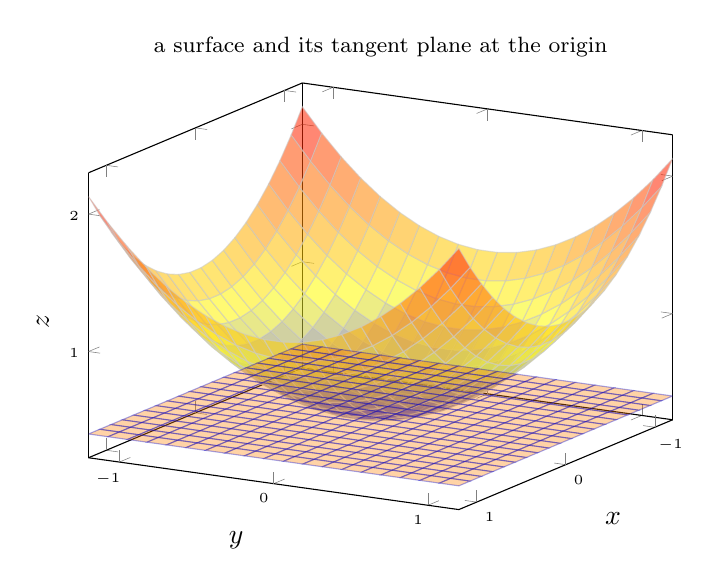
\begin{tikzpicture}
\begin{axis}[
  width=9cm, height=7cm,
  view={120}{20},
  xlabel={$x$}, ylabel={$y$}, zlabel={$z$},
  tick label style={font=\tiny},
  domain=-1.2:1.2, y domain=-1.2:1.2,
  samples=20, samples y=20,
  title={\footnotesize a surface and its tangent plane at the origin},
]
\addplot3[surf, opacity=0.55, faceted color=gray!40] {0.6*x^2 + 0.6*y^2 + 0.4};
\addplot3[surf, opacity=0.35, color=orange] {0.4 + 0*x + 0*y};
\end{axis}
\end{tikzpicture}
\caption{The bowl $z=0.6x^2+0.6y^2+0.4$ and its tangent plane at the bottom point
$(0,0,0.4)$. Because $\grad f(0,0)=(0,0)$, the tangent plane is horizontal -- the
flat ``floor'' that the bowl melts into when you zoom in on its lowest point. At a
slanted point the plane would tilt to match.}
\label{ch33:fig-plane}
\end{figure}

\begin{example}[Estimating a value without a calculator]
\label{ch33:ex-linapprox}
Estimate $\sqrt{(3.02)^2 + (3.97)^2}$ using a tangent plane.

Let $f(x,y)=\sqrt{x^2+y^2}$ and anchor at the friendly point $(a,b)=(3,4)$, where
$f(3,4)=\sqrt{9+16}=5$ exactly. The partials are
\[
  f_x = \frac{x}{\sqrt{x^2+y^2}}, \qquad f_y = \frac{y}{\sqrt{x^2+y^2}},
\]
so $f_x(3,4)=\tfrac35$ and $f_y(3,4)=\tfrac45$; thus $\grad f(3,4)=(\tfrac35,
\tfrac45)$. The steps are $\Delta x = 3.02-3 = 0.02$ and
$\Delta y = 3.97-4 = -0.03$. The linear approximation gives
\[
  f(3.02,3.97)\approx 5 + \tfrac35(0.02) + \tfrac45(-0.03)
  = 5 + 0.012 - 0.024 = 4.988.
\]
A calculator gives $\sqrt{3.02^2+3.97^2}=\sqrt{9.1204+15.7609}=\sqrt{24.8813}
\approx 4.98812$. Our tangent-plane estimate $4.988$ is correct to four decimals,
from arithmetic you can do in your head -- because near $(3,4)$ the surface is
practically its tangent plane.
\end{example}

\begin{connectionbox}
This is the engine of \emph{error propagation} in the lab. If a quantity
$f(x,y)$ is computed from two measurements $x,y$ with small uncertainties
$\Delta x,\Delta y$, then to first order the uncertainty in $f$ is
$\Delta f \approx f_x\,\Delta x + f_y\,\Delta y$. The partial derivatives are the
\emph{sensitivities}: they say how strongly each input's error feeds through to
the output. The gradient is the vector of sensitivities. Scientists who have never
heard the word ``gradient'' use this formula every time they write
``$\pm$'' after a result.
\end{connectionbox}

\section{Gradient Descent: How Machines Learn}
\label{ch33:gd}

We have all the ingredients for one of the most consequential algorithms of our
century. Here is the entire idea in one breath: \emph{to minimize a function,
keep stepping in the direction of steepest descent} -- that is, in the direction
of $-\grad f$ -- and you will walk downhill toward a valley.

\begin{applicationbox}
\textbf{Gradient descent in machine learning.} A machine-learning model has a pile
of adjustable numbers called \emph{parameters} (or weights), which we collect into
a vector $\vec w=(w_1,\dots,w_n)$ -- a modern network has millions or billions of
them. A \emph{loss function} $L(\vec w)$ measures how badly the model does on the
training data: big loss means bad predictions, small loss means good ones.
Training the model means \emph{minimizing} $L$ over the weights.

We cannot see this $n$-dimensional landscape, and we certainly cannot solve
$\grad L = \vec 0$ by hand for a billion variables. But we can do what the foggy
hiker of the earlier walkbox does. At our current weights, we compute the gradient
$\grad L(\vec w)$ -- the direction in weight-space that would increase the loss
fastest -- and we step the \emph{opposite} way:
\[
  \boxed{\;\vec w_{\text{new}} = \vec w_{\text{old}} - \eta\,\grad L(\vec
w_{\text{old}}).\;}
\]
The number $\eta>0$ is the \textbf{learning rate}, the size of the step. Repeat
millions of times and the weights slide downhill into a valley of low loss -- the
model has \emph{learned}. The gradient here is computed by the multivariable chain
rule applied layer by layer through the network; that organized application of
the chain rule is exactly what \emph{backpropagation} is. Everything in this
chapter -- gradient as steepest direction, chain rule as the way to compute it --
is precisely the mathematics that trains modern AI.
\end{applicationbox}

\begin{intuitionbox}
Why step \emph{against} the gradient? Because $-\grad L$ is the direction of
steepest \emph{descent} (Section~\ref{ch33:gradient}): of all directions you could
step, it lowers the loss the fastest. And why multiply by a small $\eta$? Because
the gradient is only the slope \emph{at your current point}; trust it only for a
short step. The linear approximation
$L(\vec w - \eta\,\grad L)\approx L(\vec w) - \eta\,\norm{\grad L}^2$ shows that as
long as $\eta$ is small and $\grad L\neq\vec 0$, the loss strictly decreases: the
term $-\eta\norm{\grad L}^2$ is negative. That single inequality is the
mathematical guarantee that a small gradient step makes progress.
\end{intuitionbox}

\begin{figure}[H]
\centering
\begin{tikzpicture}
\begin{axis}[
  width=8.4cm, height=6.6cm,
  xmin=-2.6, xmax=2.6, ymin=-2.6, ymax=2.6,
  xlabel={$w_1$}, ylabel={$w_2$},
  tick label style={font=\tiny},
  axis lines=middle,
  title={\footnotesize gradient descent on the bowl $L=w_1^2+w_2^2$},
]
\addplot[gray!55, samples=80, domain=0:360] ({2.3*cos(x)},{2.3*sin(x)});
\addplot[gray!55, samples=80, domain=0:360] ({1.6*cos(x)},{1.6*sin(x)});
\addplot[gray!55, samples=80, domain=0:360] ({0.95*cos(x)},{0.95*sin(x)});
\addplot[gray!55, samples=80, domain=0:360] ({0.45*cos(x)},{0.45*sin(x)});
\addplot[-{Stealth[length=2mm]}, tangentred, very thick] coordinates {
  (2.30,1.70) (1.47,1.09) (0.94,0.70) (0.60,0.45) (0.39,0.29) (0.25,0.18)};
\addplot[mark=*, mark size=1.5pt, black] coordinates {(2.30,1.70)};
\node[font=\tiny, anchor=west] at (axis cs:2.30,1.95) {start};
\addplot[mark=*, mark size=1.5pt, structurepurple] coordinates {(0,0)};
\node[font=\tiny, structurepurple, anchor=west] at (axis cs:0.12,-0.3) {minimum};
\end{axis}
\end{tikzpicture}
\caption{Gradient descent on $L=w_1^2+w_2^2$. Each red step points opposite the
gradient (perpendicular to the contour, straight toward the center) and is scaled
by the learning rate. The iterates march into the minimum at the origin.}
\label{ch33:fig-gd}
\end{figure}

\begin{example}[One descent step by hand]
\label{ch33:ex-gdstep}
Minimize $L(w_1,w_2)=w_1^2 + w_2^2$ starting at $\vec w_0=(2,3)$ with learning
rate $\eta=0.1$.

The gradient is $\grad L = (2w_1, 2w_2)$, so $\grad L(2,3) = (4,6)$. One step:
\[
  \vec w_1 = (2,3) - 0.1\,(4,6) = (2-0.4,\; 3-0.6) = (1.6,\,2.4).
\]
The loss dropped from $L(2,3)=4+9=13$ to $L(1.6,2.4)=2.56+5.76=8.32$. We moved
toward the origin -- the true minimum -- as expected. Notice each coordinate got
multiplied by $1-2\eta = 0.8$; iterating, the weights shrink geometrically to
zero, which is gradient descent solving this bowl exactly.
\end{example}

\begin{trapbox}
The learning rate is a genuine knife-edge. Too \emph{small} and progress is
glacial -- thousands of tiny steps. Too \emph{large} and you overshoot the valley
and bounce up the far wall; the loss can \emph{increase} and even diverge. In
Example~\ref{ch33:ex-gdstep} the update multiplied each weight by $1-2\eta$. That
factor has magnitude below $1$ (so the steps converge) only when $0<\eta<1$; at
$\eta=1$ the weights flip sign and never shrink, and for $\eta>1$ they blow up.
Choosing $\eta$ well is one of the central practical arts of training models, and
it is, at heart, the trapbox warning about trusting a linear approximation too far.
\end{trapbox}

\begin{walkbox}
Gradient descent only ever steps downhill, so it can get \emph{stuck} in a valley
that is not the lowest valley -- a \emph{local} minimum. Picture a landscape with
two basins of different depths (Figure~\ref{ch33:fig-localmin}); depending on where
you start, you slide into one or the other and stop. Why, then, does gradient descent work so astonishingly well for
training enormous neural networks, where the landscape has untold many local
minima? (A surprising partial answer modern research offers: in very high
dimensions, most of those resting points are nearly as good as the best, and true
bad traps are rare. The intuition you build here is the doorway to that research.)
\end{walkbox}

\begin{figure}[H]
\centering
\begin{tikzpicture}
\begin{axis}[
  width=10cm, height=5.2cm,
  xmin=-3.2, xmax=3.2, ymin=-1.4, ymax=3.2,
  axis lines=middle,
  xlabel={$w$}, ylabel={loss},
  tick label style={font=\tiny},
  xtick={\empty}, ytick={\empty},
  title={\footnotesize a loss landscape with two valleys of different depth},
]
% a double-well curve: f(w) = 0.18 w^4 - 1.1 w^2 - 0.35 w + 1.6
\addplot[curveblue, very thick, samples=140, domain=-3:3]
  {0.18*x^4 - 1.1*x^2 - 0.35*x + 1.6};
% shallow local minimum near w ~ -1.65
\addplot[mark=*, mark size=1.5pt, tangentred] coordinates {(-1.65,0.52)};
\node[font=\tiny, tangentred, anchor=south] at (axis cs:-1.65,0.66) {local min (trap)};
% deep global minimum near w ~ 1.75
\addplot[mark=*, mark size=1.5pt, structurepurple] coordinates {(1.75,-0.70)};
\node[font=\tiny, structurepurple, anchor=north] at (axis cs:1.75,-0.85) {global min};
% two starting balls
\addplot[mark=*, mark size=1.2pt, black] coordinates {(-2.55,2.95)};
\addplot[mark=*, mark size=1.2pt, black] coordinates {(0.55,1.09)};
\end{axis}
\end{tikzpicture}
\caption{Gradient descent only steps downhill, so where you start decides where you
stop. A ball released on the far left slides into the shallow left valley (a
\emph{local} minimum) and halts; one released just right of center rolls into the
deeper right valley (the \emph{global} minimum). Both are critical points where the
slope is zero, but only one is the true bottom.}
\label{ch33:fig-localmin}
\end{figure}

\section{Finding and Classifying Critical Points: the Hessian}
\label{ch33:hessian}

To find the peaks and valleys of a surface, we look for the places where it is
momentarily flat -- where the tangent plane is horizontal. In one variable we set
$f'(x)=0$; in several variables we set the entire gradient to zero.

\begin{definition}[Critical point]
\label{ch33:def-critical}
A point $(a,b)$ is a \textbf{critical point} of $f$ if $\grad f(a,b)=\vec 0$, that
is $f_x(a,b)=0$ and $f_y(a,b)=0$ (or if the gradient fails to exist). At such a
point the tangent plane is horizontal.
\end{definition}

A horizontal tangent plane is necessary for a local max or min -- if the ground
sloped at all, you could go uphill one way and downhill the other, so it would be
neither a top nor a bottom. But ``flat'' alone does not tell you \emph{which}.
There are three flavors of critical point, and the new one has no analogue in a
single variable.

\begin{itemize}
\item \textbf{Local minimum:} the surface curves \emph{up} in every direction -- a
bowl. You are at the bottom of a valley.
\item \textbf{Local maximum:} the surface curves \emph{down} in every direction --
a dome. You are at a summit.
\item \textbf{Saddle point:} the surface curves up in some directions and down in
others -- like a mountain pass, or the seat of a horse saddle. Up along the horse's
spine, down toward the stirrups. This is genuinely new: a point can be flat yet be
neither a max nor a min.
\end{itemize}

\begin{figure}[H]
\centering
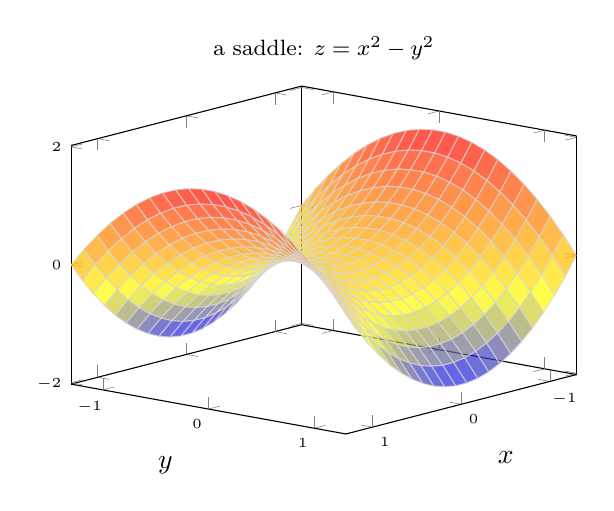
\begin{tikzpicture}
\begin{axis}[
  width=8cm, height=6cm,
  view={130}{18},
  xlabel={$x$}, ylabel={$y$},
  tick label style={font=\tiny},
  domain=-1.3:1.3, y domain=-1.3:1.3,
  samples=22, samples y=22,
  title={\footnotesize a saddle: $z=x^2-y^2$},
]
\addplot3[surf, opacity=0.7, faceted color=gray!30] {x^2 - y^2};
\end{axis}
\end{tikzpicture}
\caption{The saddle $z=x^2-y^2$ at the origin. Along the $x$-axis ($y=0$) it is the
upward parabola $z=x^2$ -- a minimum that way. Along the $y$-axis ($x=0$) it is the
downward parabola $z=-y^2$ -- a maximum that way. Flat at the origin, but neither a
peak nor a valley.}
\label{ch33:fig-saddle}
\end{figure}

\subsection{The second-derivative test, intuitively}

How do we tell the three apart without plotting? By looking at \emph{curvature} --
the second derivatives. In one variable, after $f'(a)=0$, the sign of $f''(a)$
decided max ($f''<0$, concave down) versus min ($f''>0$, concave up). In two
variables there are \emph{three} second partials to track,
\[
  f_{xx} = \pdv{}{x}\Big(\pdv{f}{x}\Big),\qquad
  f_{yy} = \pdv{}{y}\Big(\pdv{f}{y}\Big),\qquad
  f_{xy} = \pdv{}{y}\Big(\pdv{f}{x}\Big),
\]
(and for the functions we meet, $f_{xy}=f_{yx}$, the mixed partials agree). We
arrange them in a $2\times 2$ grid called the \textbf{Hessian matrix}:
\[
  H = \begin{pmatrix} f_{xx} & f_{xy} \\ f_{xy} & f_{yy}\end{pmatrix}.
\]
The Hessian is the multivariable second derivative: it records the curvature of
the surface in every direction, just as the gradient recorded the slope in every
direction. The quantity that decides the verdict is its \textbf{determinant},
\[
  D = f_{xx}f_{yy} - (f_{xy})^2.
\]

\begin{focusbox}
\textbf{The second-derivative (Hessian) test.} At a critical point $(a,b)$, let
$D = f_{xx}f_{yy} - f_{xy}^2$, all evaluated at $(a,b)$.
\begin{itemize}
\item If $D>0$ and $f_{xx}>0$: \textbf{local minimum} (a bowl, curving up).
\item If $D>0$ and $f_{xx}<0$: \textbf{local maximum} (a dome, curving down).
\item If $D<0$: \textbf{saddle point} (curving up one way, down another).
\item If $D=0$: the test is \textbf{inconclusive} -- the curvature is too gentle
to decide; look closer.
\end{itemize}
\end{focusbox}

\begin{intuitionbox}
Where does $D = f_{xx}f_{yy}-f_{xy}^2$ come from, intuitively? Two things must be
true for a genuine bowl. First, it must curve up along the $x$-direction
\emph{and} along the $y$-direction: $f_{xx}>0$ and $f_{yy}>0$. But that is not
enough -- a strong mixed term $f_{xy}$ can twist the surface so that even though
both axis-directions curve up, some diagonal direction curves \emph{down},
secretly making a saddle. The determinant $D$ is exactly the bookkeeping that
catches this twist: requiring $f_{xx}f_{yy} > f_{xy}^2$ says the genuine upward
curvature beats the twisting. When the twist wins ($D<0$), you have a saddle: up
some ways, down others. The sign of $f_{xx}$ then just picks bowl ($+$) from dome
($-$). This is the two-dimensional cousin of ``concave up vs concave down,'' with
$D$ guarding against the diagonal sabotage that one variable cannot have.
\end{intuitionbox}

\begin{whybox}
\textbf{Why the determinant decides it (the deeper reason).} Near a critical point
the gradient is zero, so the linear part of $f$ vanishes and the \emph{quadratic}
part takes over:
\[
  f(a+h,b+k) \approx f(a,b) + \tfrac12\big(f_{xx}h^2 + 2f_{xy}hk + f_{yy}k^2\big).
\]
The fate of the critical point hangs entirely on the sign of the quadratic form
$Q(h,k)=f_{xx}h^2 + 2f_{xy}hk + f_{yy}k^2$. If $Q>0$ for every direction $(h,k)$,
the surface rises every way -- a min. If $Q<0$ always -- a max. If $Q$ is positive
some ways and negative others -- a saddle. Completing the square (assuming
$f_{xx}\neq 0$),
\[
  Q = f_{xx}\Big(h + \tfrac{f_{xy}}{f_{xx}}k\Big)^2
      + \frac{f_{xx}f_{yy}-f_{xy}^2}{f_{xx}}\,k^2,
\]
and you can read off everything: the leftover coefficient on $k^2$ is $D/f_{xx}$.
For $Q$ to keep one sign, both pieces need matching signs, which forces $D>0$;
then $f_{xx}$ sets that sign (min if $+$, max if $-$). If $D<0$ the two squared
pieces fight, so $Q$ takes both signs -- a saddle. The determinant is not a magic
recipe; it is the discriminant of a quadratic form, the exact higher-dimensional
heir of the $f''$ sign test.
\end{whybox}

\begin{example}[Classifying every critical point]
\label{ch33:ex-classify}
Classify the critical points of $f(x,y)=x^3 - 3x + y^2$.

\textbf{Step 1: find them.} $f_x = 3x^2 - 3 = 3(x^2-1)$ and $f_y = 2y$. Setting
both to zero: $f_y=0$ gives $y=0$, and $f_x=0$ gives $x^2=1$, so $x=\pm 1$. Two
critical points: $(1,0)$ and $(-1,0)$.

\textbf{Step 2: second partials.} $f_{xx}=6x$, $f_{yy}=2$, $f_{xy}=0$. So
$D = f_{xx}f_{yy}-f_{xy}^2 = (6x)(2) - 0 = 12x$.

\textbf{Step 3: apply the test.}
\begin{itemize}
\item At $(1,0)$: $D = 12(1) = 12 > 0$ and $f_{xx}=6(1)=6>0$. \emph{Local
minimum.}
\item At $(-1,0)$: $D = 12(-1) = -12 < 0$. \emph{Saddle point.}
\end{itemize}
This fits the shape of $f$: in $x$ it is a cubic (one local min at $x=1$, one local
max at $x=-1$), and in $y$ it is the upward parabola $y^2$. At $x=1$ both
directions curve up -- a true bowl. At $x=-1$ the $x$-cubic curves down while the
$y$-parabola curves up -- up one way, down the other, a saddle. The Hessian test
read all of this off three derivatives.
\end{example}

\begin{example}[A clean maximum]
\label{ch33:ex-max}
Classify the critical point of $f(x,y)=4 - x^2 - y^2 + 2x$.

$f_x = -2x + 2 = 0 \Rightarrow x = 1$; $f_y = -2y = 0 \Rightarrow y = 0$. One
critical point $(1,0)$. Second partials: $f_{xx}=-2$, $f_{yy}=-2$, $f_{xy}=0$, so
$D = (-2)(-2) - 0 = 4 > 0$ with $f_{xx}=-2<0$: a \emph{local maximum}. Indeed
$f = 5-(x-1)^2 - y^2$ after completing the square, an upside-down bowl with summit
$5$ at $(1,0)$ -- exactly what the test reported.
\end{example}

\begin{historybox}
The word ``gradient'' and the $\grad$ symbol came of age in the nineteenth century.
The inverted-delta $\nabla$ was introduced by William Rowan Hamilton (around 1837)
in his work on quaternions, and the playful name \emph{nabla} -- after an ancient
Hebrew harp of similar shape -- was suggested to him by the physicist P.~G.~Tait,
who developed the operator's calculus. But the \emph{ideas} are older and grew from
physics. Joseph-Louis Lagrange and his successors were already studying the
``slope'' of potential functions, and the realization that force is the (negative)
gradient of a potential -- that nature pushes objects straight downhill on an
energy landscape -- was central to the mechanics of Lagrange, Hamilton, and later
Maxwell. The Hessian is named for Otto Hesse, who studied these determinants of
second derivatives in the 1840s while working on curves and surfaces. What we now
package neatly as ``set the gradient to zero, then check the Hessian'' was, for the
founders, the hard-won geometry of how surfaces bend -- the same geometry you have
just seen in three derivatives and one determinant.
\end{historybox}

\begin{recoverybox}
That was a lot. Here is the spine of the chapter in five sentences. (1) The
\emph{directional derivative} $D_{\vec u}f$ is the slope of $f$ as you walk in the
unit direction $\vec u$, and it equals $\grad f\cdot\vec u$. (2) The
\emph{gradient} $\grad f = (f_x,f_y)$ points in the direction of steepest ascent,
its length is the steepest slope, and it is perpendicular to level curves. (3) The
\emph{chain rule} ``multiply along paths, add across paths'' computes derivatives
through any chain of dependencies and is the engine of backpropagation. (4) Linear
approximation upgrades the tangent line to a tangent \emph{plane},
$L = f(a,b) + \grad f\cdot((x,y)-(a,b))$. (5) Critical points are where
$\grad f = \vec 0$, and the \emph{Hessian} determinant $D=f_{xx}f_{yy}-f_{xy}^2$
sorts them into minima, maxima, and the genuinely new saddles. Every item on this
list is one geometric idea -- local flatness -- seen from a different angle.
\end{recoverybox}

\section{Exercises}
\label{ch33:exercises}

\begin{exercise}[Directional derivative, by formula]
\label{ch33:exr-dir}
Let $f(x,y) = x^2 y + y^3$. Compute the directional derivative of $f$ at the point
$(2,1)$ in the direction toward $(5,5)$. (Remember to normalize the direction
vector first.)
\end{exercise}

\begin{exercise}[Steepest ascent]
\label{ch33:exr-steep}
For $f(x,y) = e^{x}\sin y$, find at the point $(0,\tfrac{\pi}{2})$: (a) the
gradient, (b) the unit direction of steepest ascent, and (c) the maximum rate of
increase. In what direction(s) is the directional derivative zero?
\end{exercise}

\begin{exercise}[Chain rule, one parameter]
\label{ch33:exr-chain1}
Let $z = x^2 - y^2$ with $x(t) = \cos t$ and $y(t) = \sin t$. Use the chain rule to
find $\dv{z}{t}$, then verify your answer by first substituting to get $z$ as an
explicit function of $t$ and differentiating directly. (You should find a clean
trigonometric expression.)
\end{exercise}

\begin{exercise}[Chain rule, two parameters]
\label{ch33:exr-chain2}
Let $z = x y$ where $x = s + t$ and $y = s - t$. Compute $\pdv{z}{s}$ and
$\pdv{z}{t}$ using the multivariable chain rule. Then compute $z$ directly in terms
of $s,t$ and confirm.
\end{exercise}

\begin{exercise}[Tangent plane and estimation]
\label{ch33:exr-plane}
Let $f(x,y) = \ln(x^2 + y^2)$. (a) Write the equation of the tangent plane to the
graph at $(1,0)$. (b) Use it to estimate $f(1.1,\,0.05)$, and compare with the true
value.
\end{exercise}

\begin{exercise}[A gradient descent run]
\label{ch33:exr-gd}
Consider $L(w_1,w_2) = w_1^2 + 4w_2^2$ with learning rate $\eta = 0.1$, starting at
$(w_1,w_2)=(1,1)$. (a) Carry out two steps of gradient descent by hand, reporting
the iterates and the loss at each. (b) Each coordinate is multiplied by a constant
factor every step -- find the two factors. Why does $w_2$ converge faster than
$w_1$, and what does that say about choosing $\eta$ when the bowl is stretched?
\end{exercise}

\begin{exercise}[Classify the critical points]
\label{ch33:exr-classify}
Find and classify all critical points of $f(x,y) = x^3 + y^3 - 3xy$ using the
Hessian test. (You should find one saddle and one local extremum.)
\end{exercise}

\begin{exercise}[The perpendicularity, concretely]
\label{ch33:exr-perp}
Let $f(x,y) = x^2 + 4y^2$, whose level curves are ellipses. At the point
$(2,1)$ (which lies on the level curve $f=8$): (a) compute $\grad f(2,1)$;
(b) find a vector tangent to the ellipse $f=8$ at $(2,1)$ (hint: parametrize, or
use implicit differentiation $\dv{y}{x}$ on $x^2+4y^2=8$); (c) verify by a dot
product that the gradient and the tangent are perpendicular.
\end{exercise}

\begin{exercise}[Conceptual: partials exist but no plane]
\label{ch33:exr-concept}
Explain in your own words, with the help of the trapbox in
Section~\ref{ch33:chain}, why ``all partial derivatives exist at a point'' is
\emph{not} enough to guarantee that the chain rule formula holds there. What
stronger condition (stated in Section~\ref{ch33:tangentplane}) is the right one,
and what does it say geometrically?
\end{exercise}

\begin{exercise}[Proof: steepest ascent]
\label{ch33:exr-proof}
Prove that among all unit vectors $\vec u$, the directional derivative
$D_{\vec u} f = \grad f \cdot \vec u$ is maximized when $\vec u$ points along
$\grad f$, and that the maximum value is $\norm{\grad f}$. (Use the
identity $\grad f \cdot \vec u = \norm{\grad f}\cos\theta$ and explain why
$\cos\theta = 1$ is forced. State clearly where you use $\norm{\vec u} = 1$.)
\end{exercise}

\begin{exercise}[Proof: gradient perpendicular to level sets]
\label{ch33:exr-proofperp}
Suppose a differentiable path $\vec r(t) = (x(t), y(t))$ lies entirely on the level
curve $f(x,y) = c$. Differentiate the identity $f(x(t),y(t)) = c$ with respect to
$t$ and use the chain rule to conclude that $\grad f \cdot \vec r\,'(t) = 0$.
Explain in one sentence why this proves $\grad f$ is perpendicular to the level
curve.
\end{exercise}
